%%%%%%%%%%%%%%%%%%%%%%%%%%%%%%%%%%%%%%%%%%%%%%%%%%%%%%%%%%%%%%%%
%% Front page of my Ph.D. thesis
%% (C) Copyright 1997 by Kenneth Geisshirt (kneth@chem.ruc.dk)
%% Last modified: 8 January 1998
%%%%%%%%%%%%%%%%%%%%%%%%%%%%%%%%%%%%%%%%%%%%%%%%%%%%%%%%%%%%%%%%

\thispagestyle{empty}
\begin{center}
  {\Huge Non-Equilibrium Molecular Dynamics Simulations: \\ Application to \\
Oscillating Chemical Reactions \\ and \vspace{0.15cm} \\ Inelastic Colliding Particles}
\end{center}

\vspace{0.25cm}
\begin{center}
  {\large A Ph.D.\ thesis in Chemistry/Soft Material Science, December 1997}
\end{center}

\vfill

\begin{minipage}[b]{0.46\linewidth}
  \centering\epsfig{file=Frontpage/early.ps,width=\linewidth,height=\linewidth}
\end{minipage}\hfill
\begin{minipage}[b]{0.46\linewidth}
  \centering\epsfig{file=Frontpage/late.ps,width=\linewidth,height=\linewidth}
\end{minipage}

\vfill

\begin{minipage}[c]{3cm}
  
\epsfig{file=Frontpage/logo.ps,width=2.5cm,angle=270}
\end{minipage}\hfill
\begin{minipage}[c]{10cm}
  Kenneth Geisshirt \\
  Department of Life Sciences and Chemistry \\
  Roskilde University \\
  E-mail: \texttt{kneth@chem.ruc.dk}
\end{minipage}


\newpage
\thispagestyle{empty}
The pictures on the front page are snapshots from simulations of a
two-component Lennard-Jones system above and below the critical
temperature.

\vspace{1cm}
The thesis was produced using freeware only. The text was typeset using
\LaTeX, the graphs were produced by \texttt{GNUplot} and \texttt{ACEgr},
and the drawings were drawn in \texttt{xfig}. The final PostScript file
was processed on a pc running Linux.

\vfill
\copyright{} Copyright 1997 by Kenneth Geisshirt and Roskilde University
\newpage
\thispagestyle{empty}
